% Requires running Bibtex

\documentclass[%
reprint,
amsmath,amssymb,
aps,
]{revtex4-2}

\usepackage{graphicx}% Include figure files
\usepackage{dcolumn}% Align table columns on decimal point
\usepackage{bm}% bold math
\usepackage{hyperref}% add hypertext capabilities
\usepackage[font=scriptsize,labelfont=bf, justification=justified]{caption}% change fontsize in captions
\usepackage{booktabs}% cool table style
\hypersetup{
	colorlinks=true,       % false: boxed links; true: colored links
	linkcolor=black,        % color of internal links
	citecolor=black,        % color of links to bibliography
	filecolor=black,     % color of file links
	urlcolor=black         
}

\usepackage{bibspacing}
\setlength{\bibitemsep}{.5\baselineskip plus .05\baselineskip minus .05\baselineskip}


\begin{document}
	
	\preprint{APS/123-QED}
	
	\title{PHYC30170 Physics with Astronomy and Space Science Lab 1;\\An Investigation of Surface Plasmon Resonance}
	
	\author{Daragh Hollman}
	\email{daragh.hollman@ucdconnect.ie}
	
	\date{\today}
	
	\begin{abstract}
		The aims of this experiment were to determine the excitation angle of the surface plasmon within the Kretschmann configuration and to investigate the dependence of surface plasmon resonance (SPR) on the wavelength of the incident light and the thickness of the silver foil. [NOT FINISHED]
	\end{abstract}

	\maketitle
	
	\section{Introduction}		
		Surface plasmons are transverse magnetic waves, comprised of oscillating electrons, which travel along the boundary of a metal and a dielectric \cite{undergradToledo}. They were first discovered in 1957 by R. H. Ritchie The study of surface plasmons is very important and has many applications in biophysics, particularly in the analysis of biomolecular interactions \cite{biomedicalApplications}, and in many fields of optics including but not limited to sub-wavelength optics and near-field optics \cite{opticalApplications}.
	
	\section{Theory}
		\subsection{Excitation of Free Electrons}
			\url{https://iopscience-iop-org.ucd.idm.oclc.org/article/10.1088/0022-3727/45/11/113001}
		
		\subsection{Surface Plasmon Waves}
		
		\subsection{Apparatus}
			The apparatus was set up as shown in figure \ref{fig:apparatus}. More specifically, the Kretschmann configuration was used, figure \ref{fig:kConfig}.
			
			\begin{figure}
				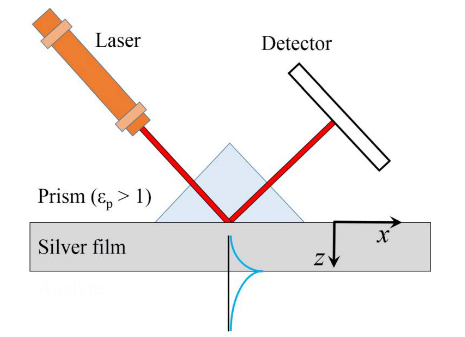
\includegraphics[width=0.9\columnwidth]{kConfig.png}
				\caption{\label{fig:kConfig} The Kretschmann configuration. The silver film was evaporated onto the glass prism. The light from the laser excites the plasmons on the outer side of the film. \cite{opticalApplications}}
			\end{figure}
	 
	\section{Methodology}
		\subsection{Apparatus Setup}
			The apparatus was set up in the Kretschmann configuration as shown in figure \ref{fig:kConfig}. A silver film was evaporated onto three prisms so that the thickness of the film could be varied. Thicknesses of 10nm, 13nm, and 15nm were used. The prism was placed in the centre of a bidirectional stepping rotary table. This table had two independently movable discs (specifically one disc and one annulus) controlled by stepper motors which, through a gear system, had a precision of $0.045$ degrees per step. The prism was placed on the inner disc and a photodiode was fixed on the outer annulus to be used as a detector.\\
			
			The apparatus was controlled using python to interface with a USB multifunction I/O device, NI USB-6009 \cite{nationalInstruments}. This was used as a digital to analogue converter to control the stepper motors as well as an input from the photodiode to read voltages.

			\subsubsection{Light Source}
				Three He-Ne lasers were used of wavelengths 633nm, 515nm, and 405nm all of which had a maximum power $\le 4 \,\text{mW}$. In this report we will refer to these lasers as red, green, and blue respectively. A linear polarising filter was positioned between the laser and the prism such to p-polarise the incident light.
			
			\subsubsection{Motor Programming}
				Be salty about things being labelled incorrectly.
				
				How were the motors powered
			
			\subsubsection{Developing an Algorithm for Data Collection}
				Note efficiency
			
			\subsubsection{Laser Alignment}
			
		\subsection{Data Collection}
			\subsubsection{}
		
		
	
	\section{Results and Analysis}
		\subsection{Varying Laser Wavelength}
		
		\subsection{Varying Metal Thickness}
	
		\subsection{Anomaly found during Red Laser Runs}

	\section{Conclusion}
		
		
	\newpage
	\bibliography{surfacePlasmons}% Produces the bibliography via BibTeX.
		
	\newpage
	\appendix
		
		
\end{document}

